\documentclass{svproc}
\usepackage{newtxmath}
\usepackage{fontspec}
\setmainfont{Times New Roman}
\usepackage{microtype}
\setlength{\emergencystretch}{2em}
\usepackage{url}
\def\UrlFont{\rmfamily}
\usepackage{graphicx,booktabs,amsmath}
\usepackage{algorithm,algorithmic}
\usepackage{placeins}
\usepackage[hidelinks]{hyperref}
\hypersetup{pdfauthor={},pdftitle={When Tool Agreement Is Not Enough},pdfsubject={Anonymous IntelliSys 2027 research draft}}
\begin{document}
\mainmatter
\title{When Tool Agreement Is Not Enough: Budgeted Recovery and Silent-Error Acceptance in Intelligent Workflows}
\titlerunning{Budgeted Recovery and Silent-Error Acceptance}
\author{}
\authorrunning{}
\institute{}
\maketitle
\begin{abstract}
Intelligent workflows must decide whether to accept a tool response, retry a failed call, switch tools, or request verification. These choices are often compared without distinguishing visible errors from mutually consistent wrong answers. We study this distinction using executed SQLite, Python, and NumPy computations on three public datasets. A new workload contains 72 development and 72 test queries across four aggregation families. Nine controllers operate under hard budgets of one, two, or three engine invocations; repeated fault schedules are paired across policies. Development choices are frozen before the main evaluation. Retry handles transient errors, while switching also handles persistent primary-engine errors. Under independent corruptions with distinct wrong values, three-call agreement answers 94.4\% correctly and abstains on the remainder. A subsequent exploratory sensitivity allows independent failures to return the same wrong value: correctness is unchanged, but the 5.6\% abstention rate becomes wrong-answer acceptance. Under increased corruption this rate reaches 16.4\%, exceeding the development-selected single engine's 14.9\%. Shared corruption defeats every agreement policy. Development tuning selects full verification rather than a selective gate, providing no evidence of an adaptive-gating advantage. The contribution is a controlled empirical separation of recovery, verification, and error-value diversity, with explicit limits from authored queries and injected local faults.
\keywords{Intelligent workflows, Tool verification, Fault injection, Recovery, Decision-making systems}
\end{abstract}

\section{Introduction}
A successful tool invocation does not establish that its response is correct. A database can return an error, a computation can return an incorrect scalar, or several components can return the same incorrect scalar. An intelligent workflow controller must decide what to do with these different observations while respecting a resource limit. Retrying, switching tools, and requiring agreement allocate resources differently and provide different kinds of evidence.

This paper studies the acceptance decision after execution, rather than predicting an operation set from task wording. The motivating question is: \emph{under a fixed invocation budget, when does another tool response justify accepting an answer?} The distinction matters because agreement is informative only relative to assumptions about the errors that the components can share. A second successful response can corroborate a result or repeat the same mistake.

\paragraph{Toward Foundational Tool-Use Control.}
Modern intelligent systems use language-model agents to orchestrate tools, APIs, and computational engines \cite{yao2023react,xiang2026scheduler}. Full agent loops combine controller decisions with language interpretation, stochastic generation, planning, and response parsing. This coupling can make it difficult to distinguish a faulty acceptance rule from an upstream interpretation error.

We therefore present a \emph{controlled, foundational lower-bound study} of the control layer: real numerical engines execute structured queries while the controller allocates a fixed invocation budget $K\in\{1,2,3\}$. Here ``lower-bound'' denotes a deliberately simplified engineering test, not a mathematical lower bound on LLM-agent reliability. The engines are deterministic in fault-free operation; reproducible fault interventions supply the uncertainty. This design isolates whether retry, switching, and verification rules use the available evidence appropriately before adding the further variability of a language-model agent. It provides an auditable precursor to full agent evaluation, while leaving transfer to stochastic LLM-driven workflows untested.

We examine this question with real numerical engines over public tabular data. Structured queries are executed through SQLite, Python reductions, and NumPy. A controlled wrapper injects explicit database exceptions and silent numeric corruptions. Controllers receive the query, their remaining budget, and observed status/value pairs. They cannot see the fault regime, injection state, or evaluation target. Exact invocation counts, including failed calls, replace a manually weighted operation-cost model.

Three questions guide the study. \textbf{RQ1:} Which observed failures are repaired by retrying or switching, and do these recovery mechanisms address silent errors? \textbf{RQ2:} At equal hard call caps, does a development-tuned verification gate improve on capable single-engine, agreement, and majority baselines? \textbf{RQ3:} How do increased corruption, coinciding wrong values, and shared faults change the evidence provided by agreement?

The contribution is an empirical evaluation contract and a set of paired comparisons, not a new learning or voting algorithm. The experiments expose a construction-sensitive result: distinct injected wrong values produce zero accepted errors under agreement, but permitting the same wrong value converts abstentions into incorrect answers without changing correctness. The development gate also collapses to always verifying when affordable. These negative findings prevent attributing reliability to adaptive gating or engine diversity alone.

\section{Related Work and Study Boundary}
The dependence of redundant software on its failure structure is established. Knight and Leveson experimentally challenged the assumption that separately developed programs fail independently \cite{knight1986}. Our work does not rediscover that principle. It applies the distinction between error incidence and wrong-value agreement to a bounded workflow acceptance interface with measured invocation counts.

Modern agent studies make the operational question timely. ToolMaze evaluates dynamic replanning under explicit and implicit perturbations \cite{toolmaze2026}. MCP-Injector introduces protocol-aware tool-call fault injection with different persistence patterns \cite{mcp2026}. ReliabilityBench studies repeated execution, perturbations, and tool/API failures \cite{reliability2026}. These are broader agent evaluations; our study isolates the controller's acceptance, abstention, and extra-call decisions without a language model. We neither reproduce their agent results nor compare numerical performance across incompatible tasks.

ReAct interleaves reasoning and environmental action \cite{yao2023react}, while ToolSandbox supports stateful evaluation of tool use \cite{lu2025toolsandbox}. LLM-as-Scheduler studies dynamic workflow scheduling \cite{xiang2026scheduler}. These systems motivate response-conditioned control, but our structured queries require neither natural-language interpretation nor learned planning. The evaluated policies are transparent recovery and verification rules.

A related anonymous manuscript studies pre-execution operation selection on synthetic tasks \cite{relatedSubmission}. The present work uses disjoint query tasks, public data, different executed engines, a response-conditioned policy interface, and new experiments. It does not reuse the companion manuscript's classifiers, task labels, or numerical results. The relation is the broader workflow-control motivation; submission-overlap assessment requires considering both complete manuscripts.

\section{Decision Contract and Failure Model}
\subsection{Observations and Hard Budgets}
A task $q$ specifies an aggregation, a target feature, a filter feature, and a numeric threshold. A controller chooses an engine $e_t$ or terminates after observing history
\begin{equation}
h_t=\bigl((e_1,s_1,v_1),\ldots,(e_t,s_t,v_t)\bigr),
\end{equation}
where status $s_i$ is success or error and $v_i$ is a scalar or absent. It may accept one observed value or abstain. Every invocation consumes one unit, including an exception. The environment rejects calls beyond $K\in\{1,2,3\}$. There are no free verifier or fallback calls.

An offline Decimal implementation computes reference answer $y_q$ from the original numeric strings. This reference is inaccessible to the controller. A returned scalar is correct when its absolute difference from the reference is at most $10^{-6}$ or its relative difference is at most $10^{-9}$. The same tolerance determines agreement. Define correct, wrong, and abstained indicators as $C,W,Z$, with $C+W+Z=1$. Correctness is an executed numerical outcome, not agreement with a route label.

\begin{figure}[!htbp]
\centering
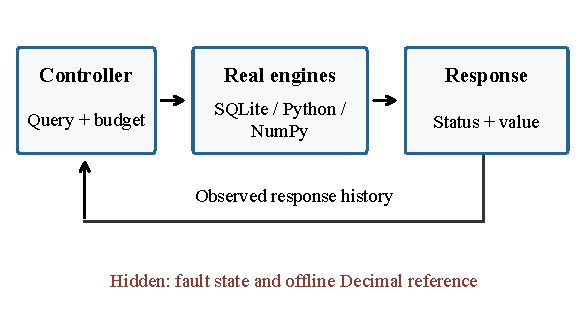
\includegraphics[width=\textwidth]{figures/recovery_contract.pdf}
\caption{Controllers observe tool responses; fault state and the reference remain hidden.}
\label{fig:contract}
\end{figure}

Figure~\ref{fig:contract} shows the separation between the response interface and offline evaluation. Engine names and query metadata are equally available to all policies. No prompt contains an outage marker, and no controller receives the regime label. The hidden schedule is paired across policies using query, fault seed, engine, and attempt identity.

\subsection{Why Agreement Needs an Error Model}
Two components can agree either on the reference value or on an erroneous value. In particular,
\begin{equation}
P(\text{wrong agreement})=\sum_{v\ne y_q}P(v_1=v,\ v_2=v).
\label{eq:wrongagreement}
\end{equation}
Independent error events do not imply that the erroneous values are distinct. If each component returns the same wrong scalar when corrupted, wrong agreement can occur even when the corruption indicators are independent. Conversely, assigning a unique wrong offset to each engine makes wrong agreement impossible by construction in the absence of collisions with the reference.

For three independent binary corruption indicators with probabilities $p_1,p_2,p_3$, all returning one shared wrong value, the probability of an incorrect majority is
\begin{equation}
p_1p_2+p_1p_3+p_2p_3-2p_1p_2p_3.
\end{equation}
This elementary voting calculation motivates testing the error-value model separately from the event-dependence model. It is not a novel theoretical result or a model of production fault rates.

The main shared-corruption intervention provides a second analytical check. Let $E$ be the event that every response equals the same incorrect scalar, with $P(E)=q$, and suppose all engines return the reference otherwise. For a controller that accepts the mutually consistent response in both cases,
\begin{equation}
P(W)=q,\qquad P(C)=1-q.
\label{eq:shared}
\end{equation}
An additional matching response supplies no distinguishing evidence under this observation model. A controller could instead abstain, so Eq.~\ref{eq:shared} is not a universal impossibility bound for every possible policy. It explains the boundary condition tested prospectively in the main evaluation; the later collision extension examines the distinct case of independent corruption events with coinciding wrong values.

\section{Data, Queries, and Executed Engines}
\subsection{Public Data and Authored Queries}
We use UCI Iris, Wine, and Banknote Authentication \cite{iris,wine,banknote}. They contain 150, 178, and 1,372 records, respectively, with four, thirteen, and four numeric features. Classification targets are excluded. Raw archives are retained unchanged and hashed. UCI distributes the datasets under CC BY 4.0; dataset attribution is preserved in the artifact.

The tasks apply COUNT, SUM, MEAN, or MAX to a selected numeric feature after filtering another feature. For each operation, three target-feature choices and two threshold choices produce 24 queries per dataset per split. Development thresholds use observed .25 and .75 order-statistic quantiles; test thresholds use .35 and .65. There are 72 development and 72 test queries, drawn from four authored query families. The task definition is structured, so results do not evaluate language understanding or paraphrase robustness.

These are real data records, but the query generator is authored for the study. Public dataset provenance does not make the tasks an independently authored benchmark. Several queries can share answer values, and the limited grammar constrains interpretation of query-cluster intervals. Ten fault seeds are repeated measurements of each query, not ten new tasks.

\subsection{Engine Implementations}
SQLite executes parameterized aggregate queries against an in-memory table. The Python implementation filters ordinary numeric lists and uses length, maximum, or \texttt{math.fsum}; NumPy uses array filtering and its reductions. Before faulted evaluation, every engine/query combination is checked against the Decimal reference. All 432 clean engine/query combinations across both splits agree within tolerance.

Every recorded invocation executes its engine; the study does not simulate success from annotated labels or reuse cached output as a new call. Nevertheless, all implementations run in one local Python process and share underlying data. They are distinct computational implementations, not independent infrastructure or evidence sources. Local timing measures this implementation and excludes remote-service and language-model latency.

\subsection{Main Fault Regimes}
\begin{table}[!htbp]
\caption{Main fault interventions; labels are hidden from controllers.}
\label{tab:regimes}
\centering\small
\begin{tabular}{p{.20\textwidth}p{.71\textwidth}}
\toprule
Regime & Intervention \\
\midrule
Clean & No injection; each engine executes its ordinary computation. \\
Transient & SQLite first attempt raises an exception; a retry can succeed. \\
Persistent & Every SQLite attempt raises an exception; alternatives work. \\
Independent & Family-dependent, persistent per-engine corruption; distinct wrong offsets. \\
Shifted & Independent corruption probabilities doubled; offsets unchanged. \\
Correlated & One shared event adds the same offset to every engine response. \\
\bottomrule
\end{tabular}
\end{table}

Table~\ref{tab:regimes} defines the main interventions. For explicit faults, SQLite actually executes against a nonexistent table, producing an operational exception. A transient fault affects its first attempt; a persistent fault affects every SQLite attempt. Alternative engines remain healthy in those regimes, making primary-engine avoidance a strong baseline.

For independent silent faults, each engine first computes its answer. A seeded wrapper then adds an engine-specific offset of 5, 7, or 11 when that engine is corrupted. The SQLite probabilities are .02, .12, .24, and .36 for COUNT, SUM, MEAN, and MAX; Python uses half those rates and NumPy uses .4 times those rates. Shifted faults double the probabilities. Corruption persists across retries within an episode. These are selected stress conditions, not estimates of how often the engines naturally fail.

The common-mode regime corrupts all responses by the same offset of 7 under a shared Bernoulli event with probability .25. Otherwise responses are clean. This intentionally creates undetectable agreement using only the permitted observations. It is a boundary condition, not an empirical discovery that NumPy and SQLite naturally share that failure rate.

\section{Controllers and Development Selection}
\subsection{Capable Fixed and Response-Conditioned Baselines}
Three \emph{single-engine} controls invoke SQLite, Python, or NumPy once. \emph{Retry} begins with SQLite and repeats it only after explicit errors, stopping at the first successful response. \emph{Switch} also begins with SQLite, but moves to Python and then NumPy after errors. Neither checks a successful scalar for silent corruption.

\emph{Agreement} begins with SQLite and requests Python when the budget permits. It accepts two agreeing values; if successful responses conflict and a third call is affordable, it requests NumPy. Two matching values are accepted; unresolved disagreement causes abstention. A single successful fallback after an explicit error is accepted because it is the only numerical evidence obtained. With $K=1$, the policy returns the primary result. These choices are disclosed so fallback coverage is not confused with a strict two-vote guarantee.

\emph{Fixed majority} spends all $K$ calls on distinct engines. At $K\geq2$ it requires at least two matching successful values; otherwise it abstains. At $K=1$ it accepts the primary result. Agreement can stop after its second call, whereas fixed majority always uses three calls when $K=3$. Both are capable multi-call alternatives, rather than intentionally restricted one-operation controls.

\subsection{Risk Gate and Selected Fixed Policy}
The \emph{risk gate} estimates the primary engine's silent-error rate by query family from successful development responses. After primary success, it accepts immediately when the estimated rate does not exceed threshold $\theta$; otherwise it follows the agreement procedure. Explicit errors trigger the same fallback behavior. No test labels or regime identities are used for this decision.

For each budget, development selects $\theta\in\{0,.05,.10,.20,1\}$ to maximize
\begin{equation}
U=C-4W-.05N,
\label{eq:utility}
\end{equation}
where $N$ is actual calls. Ties prefer a higher threshold. This is a declared illustrative utility, not an elicited user preference or a deployment safety standard. Correctness, wrong answers, abstention, and calls are reported separately to expose its trade-offs.

A \emph{development-selected fixed} control chooses among all seven base policies using the same utility and development distribution, separately for each budget. It is not given the test regime. This comparator tests whether the additional gate improves over an already capable policy selected without test knowledge.

\section{Protocol, Provenance, and Statistical Unit}
\subsection{Prospective Main Evaluation}
Development uses the clean, transient, persistent, and independent regimes, with equal weight and ten fault seeds per query. The local protocol, source fingerprints, generated query file, gate thresholds, and fixed-policy choices are recorded before the first main test evaluation. Increased corruption and common-mode faults are excluded from development. The record is local prospective evidence, not externally registered or independently timestamped preregistration.

The main evaluation executes nine policies at three budgets on 72 test queries, ten seeds, and six regimes: 116,640 policy episodes. This count must not be interpreted as 116,640 independent tasks. For paired inference, seeds are averaged within each query and differences are bootstrapped over queries within each dataset, with 1,000 resamples and a fixed random seed. Each dataset contributes equal weight. These intervals describe the authored query suite under stipulated fault schedules; three datasets and four families do not identify uncertainty over real applications generally.

\subsection{Exploratory Boundary-Condition Analysis}
After inspecting the main run, we added an exploratory \emph{collision sensitivity}: keep the independent corruption events unchanged but make every corrupted engine return its true value plus 7. Both nominal and doubled rates are evaluated. The original fitted policies remain frozen, and the source/addendum hashes are saved before this extension. Its 38,880 additional episodes are reported separately from the prospective main evaluation. This extension addresses the structural zero-error property of the initial distinct-offset model; it is not presented as an untouched confirmatory test. Its motivation is analytical: Eq.~\ref{eq:wrongagreement} already permits independent failures to agree on a wrong value. That mechanism does not depend on when the extension was designed, but its particular observed rates remain exploratory. The six main regimes and their frozen selection record are unchanged; the extension neither replaces the main evaluation nor supplies a newly independent holdout.

\section{Results}
\subsection{RQ1: Explicit Recovery Does Not Detect Silent Errors}
All single engines are correct in the clean condition. SQLite-only abstains on every explicitly faulted episode. With at least two calls, retry solves the transient cases but not the persistent cases. Switching solves both by using a healthy alternative. With three calls, persistent retry spends all three and still abstains; switching succeeds after two.

The development-selected fixed policy is NumPy alone for every budget. It solves clean and explicit-fault conditions using one call, because those interventions target SQLite. Thus successful recovery does not imply superiority to choosing an unaffected primary engine. This baseline advantage follows from the disclosed intervention model, rather than an inferred general ranking of the engines.

Under nominal independent silent faults, retry and switching both accept the initial SQLite value and achieve 81.8\% correct and 18.2\% wrong. Their behavior is identical to SQLite-only because the wrapper returns successful status. Extra allowed calls provide no protection unless the controller actually spends them checking a successful response.

\subsection{RQ2: Verification Trades Calls and Coverage}
\begin{table}[!htbp]
\caption{Three-call results: percentages of correct, wrong, and abstained episodes.}
\label{tab:main}
\centering\small
\begin{tabular}{llrrrr}
\toprule
Faults & Policy & Correct & Wrong & Abstain & Calls \\
\midrule
Independent & Selected single engine & 91.9 & 8.1 & 0.0 & 1.000 \\
Independent & Retry / switch / SQLite & 81.8 & 18.2 & 0.0 & 1.000 \\
Independent & Agreement / fitted gate & 94.4 & 0.0 & 5.6 & 2.257 \\
Independent & Fixed majority & 94.4 & 0.0 & 5.6 & 3.000 \\
Doubled & Selected single engine & 85.1 & 14.9 & 0.0 & 1.000 \\
Doubled & Retry / switch / SQLite & 62.6 & 37.4 & 0.0 & 1.000 \\
Doubled & Agreement / fitted gate & 83.6 & 0.0 & 16.4 & 2.471 \\
Doubled & Fixed majority & 83.6 & 0.0 & 16.4 & 3.000 \\
\bottomrule
\end{tabular}
\end{table}

Table~\ref{tab:main} shows the three-call comparison. In the distinct-offset independent regime, agreement achieves 94.4\% correct, zero wrong, and 5.6\% abstention, using 2.257 calls on average. The selected NumPy baseline achieves 91.9\% correct and 8.1\% wrong with one call. The paired correctness difference is 2.5 percentage points, with a query-bootstrap 95\% interval of [0.28,4.72] points. The wrong-answer difference is $-8.06$ points, with interval [$-10.28$,$-6.11$]. These intervals are conditional on the authored query/fault design.

At two calls, agreement instead achieves 74.3\% correct and abstains on 25.7\%, because a disagreement cannot be resolved. Under doubled rates, its two-call correctness is 52.9\% with 47.1\% abstention. At three calls, correctness increases to 83.6\% and abstention falls to 16.4\%. The NumPy baseline retains 85.1\% correct under doubled rates, with 14.9\% wrong. More verification therefore reduces accepted errors in this distinct-offset model while sometimes reducing the fraction answered correctly.

The fitted family risks are .011 for COUNT, .044 for SUM, .108 for MEAN, and .192 for MAX. Nevertheless, development selects threshold zero at budgets two and three. Every family has positive estimated risk, so the gate verifies every successful primary response. At budget one it selects threshold one, but cannot verify anyway. The risk gate consequently matches simple agreement in every evaluated outcome. This is evidence against a selective-gating contribution under the tested distribution and utility.

Fixed majority matches agreement's outcomes in the three-call silent regimes but always spends three calls. Agreement saves .743 calls per nominal independent episode and .529 calls under doubled rates by terminating when the first two values agree. This is the expected benefit of early stopping in an agreement procedure, not evidence that the fitted gate learns a superior acceptance policy.

\begin{figure}[!htbp]
\centering
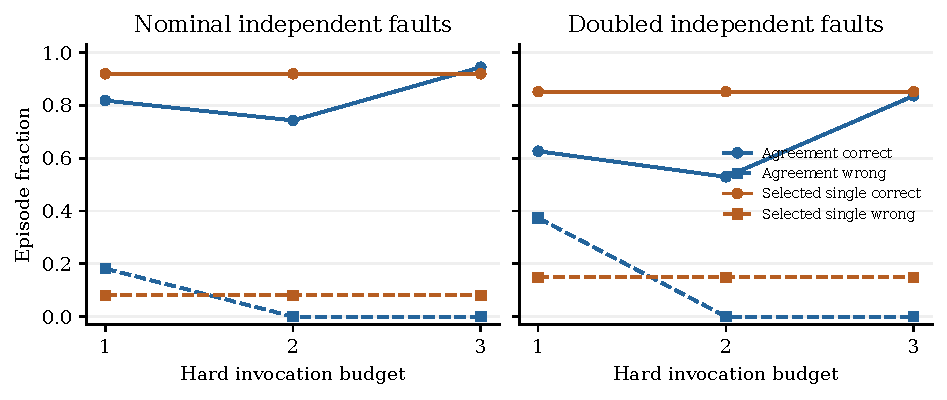
\includegraphics[width=\textwidth]{figures/budget_outcomes.pdf}
\caption{Call caps change correctness and accepted errors under distinct offsets.}
\label{fig:budgets}
\end{figure}

Figure~\ref{fig:budgets} shows the outcomes across hard call caps. The single-engine baseline has unused capacity at larger caps; this is allowed for every policy. Agreement changes behavior because another invocation can resolve a disagreement. It is the spending decision, rather than the nominal cap alone, that changes the result.

\FloatBarrier
\subsection{RQ3: Wrong-Value Diversity Changes the Meaning of Agreement}
\begin{table}[!htbp]
\caption{Agreement outcomes and selected single-engine wrong-answer rates.}
\label{tab:collision}
\centering\small
\begin{tabular}{lrrrr}
\toprule
Error model & Correct & Wrong & Abstain & Single wrong \\
\midrule
Distinct, nominal & 94.4 & 0.0 & 5.6 & 8.1 \\
Colliding, nominal & 94.4 & 5.6 & 0.0 & 8.1 \\
Distinct, doubled & 83.6 & 0.0 & 16.4 & 14.9 \\
Colliding, doubled & 83.6 & 16.4 & 0.0 & 14.9 \\
Shared event & 73.2 & 26.8 & 0.0 & 26.8 \\
\bottomrule
\end{tabular}
\end{table}

The zero wrong-answer rate above follows partly from assigning distinct erroneous offsets to the engines. It should not be interpreted as a discovered reliability guarantee. Table~\ref{tab:collision} separates prospective main rows (M) from exploratory extension rows (E). Only the E rows change the independent-offset model; they preserve the same corruption events and frozen policies, isolating whether the erroneous values coincide.

In the collision sensitivity, agreement's nominal correctness remains 94.4\%, but its 5.6\% abstention becomes 5.6\% wrong-answer acceptance. With doubled corruption, correctness remains 83.6\% while all 16.4\% previously unresolved episodes become accepted wrong answers. That wrong-answer rate exceeds the selected single engine's 14.9\%. Redundancy can therefore be less reliable than the strongest single engine under this tested collision model. The extension is exploratory and requires independent replication before broader claims.

In the prospective shared-corruption regime, all policies accept the same corrupted value whenever the latent event occurs. Observed wrong-answer acceptance is 26.8\% across the 720 query-seed episodes, with no abstention. Agreement uses two calls and fixed majority uses three, while NumPy alone uses one. The extra calls provide no distinguishing evidence because the observations agree by intervention design. Equation~\ref{eq:shared} predicts an expected wrong-answer rate of 25\% for these accepting policies; the observed 26.8\% is the finite-sample realization, not an estimate of a natural production failure rate. This prospective shared-fault result establishes the modeled boundary independently of the later collision sensitivity.

\begin{figure}[!htbp]
\centering
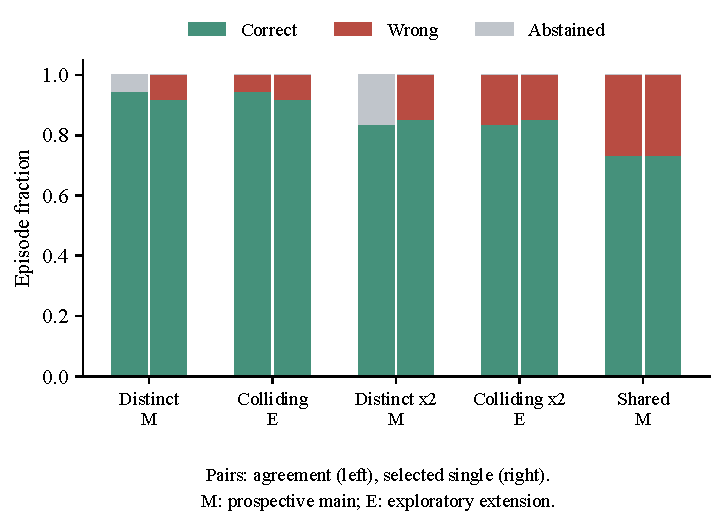
\includegraphics[width=\textwidth]{figures/error_structure.pdf}
\caption{Error structure changes accepted errors, even at the same correctness.}
\label{fig:errors}
\end{figure}

Figure~\ref{fig:errors} summarizes the distinction between error-event independence and output diversity. The engine implementations are different, but agreement remains a relation among observed values. It does not by itself identify a correct value or an independent evidence source.

\FloatBarrier
\section{Discussion and Limitations}
\subsection{What the Experiment Establishes}
The controlled interventions distinguish three mechanisms. Retrying addresses a transient explicit failure. Switching addresses a primary-engine failure when another engine works. Agreement addresses conflicting successful responses only insofar as the error model makes those conflicts informative. A call budget constrains each mechanism differently, and a lower wrong-answer rate can be purchased through abstention rather than better answer production.

The appropriate comparison is consequently a vector of correctness, wrong acceptance, coverage, and calls. The chosen utility offers one way to select a development policy, but not a universal ranking. Its selection of the one-call NumPy baseline and collapse of the gate to full verification are central results, not implementation details to omit from the comparison.

The study's narrow contribution is making the acceptance assumptions testable in one response interface. Error-value collisions explain why a seemingly strong zero-error finding can depend on the injector rather than the controller. This supports auditing fault models alongside policies when interpreting tool-reliability experiments, consistent with established warnings about software failure dependence \cite{knight1986}.

\paragraph{Implications for System Designers.}
System designers should treat multi-engine agreement as evidence conditional on fault diversity and document shared data sources, transformations, and failure modes. Candidate safeguards include semantic checks on the requested computation and invariant-based assertions, such as range or schema checks and nonincreasing counts under stricter filters, alongside genuinely independent data or computation paths. These checks must be evaluated and their invocation costs included in the acceptance budget; they are actionable design hypotheses, not mitigations validated by the present experiments.

\subsection{Limits on Transfer and Causality}
The engines execute real computations on externally sourced records, but their failures are injected. Neither additive offsets nor the chosen frequencies are calibrated to production incidents. The shared offset deliberately makes the observation histories indistinguishable from consistent answers; its failure result is a boundary check, not a newly measured operational risk.

Only SQLite receives explicit exceptions, and NumPy has the lowest specified independent-corruption rate. The selected baseline's strength therefore reflects the experimental environment. It would be inappropriate to infer that NumPy is generally more reliable than SQL, or that avoiding SQLite is a deployment recommendation. Larger fault-type and endpoint studies are needed.

The task grammar has four aggregation families, three datasets, and no natural-language interpretation. Public data are not independent task authorship. The bootstrap treats authored queries as clusters while averaging seeds; correlated semantics among queries and shared datasets still limit inference. Episode volume cannot replace query, domain, or fault diversity.

All components run locally in a shared process. Cross-engine verification is not independent-source verification, and invocation counts do not measure tokens, dollars, or remote latency. There is no LLM baseline because the study evaluates numerical acceptance control rather than language-model competence. Results should not be generalized to autonomous planning or multi-agent reasoning.

The prospective main protocol reduces test-driven tuning, but the collision extension was motivated by inspecting the first run and is explicitly exploratory. Human-author review and independently authored replication remain required for stronger scientific conclusions. Neither a rewritten framing nor new results alone establish compliance with concurrent-submission policies.

\section{Conclusion}
A workflow's response to failure depends on what it can observe and afford. In this controlled study, retry and switching repair different explicit failures; neither detects a successful but corrupted response. Verification reduces accepted errors under distinct wrong outputs, yet the same independent failure events produce accepted mistakes when erroneous values coincide. Shared corruption removes the benefit of agreement entirely.

The development-tuned gate does not outperform the simple agreement baseline, and the strongest selected single engine remains competitive. These findings define the contribution: an inspectable comparison of acceptance, recovery, and abstention under hard invocation budgets, with the fault model and its construction effects reported alongside outcomes. By abstracting away LLM stochasticity, this study supplies a controlled baseline for deterministic workflow decisions; extending the same budgeted acceptance contract to stochastic agent-driven environments is an important direction for future research.

\section*{Declaration on Generative AI}
Generative AI tools assisted study-design development, implementation, experimental analysis, manuscript drafting, language refinement, and figure preparation. The results are produced by the released executable artifacts. Human authors must critically review the research design, arguments, conclusions, code, and manuscript before submission and remain accountable for their accuracy and originality. This draft requires that human review before submission; the disclosure does not assert that it has been completed.

\section*{Data and Ethical Considerations}
The study uses attributed public numerical datasets and local read-only analytical tasks. It does not act on external services or make financial, medical, or authentication decisions. Dataset labels are excluded from computation. Identifying author information and acknowledgments are omitted for double-blind review.

\bibliographystyle{splncs03}
\bibliography{references}
\end{document}
